\documentclass[svgnames, 12pt]{beamer}

\usepackage[utf8]{inputenc}
\usepackage[english]{babel}
\usepackage[L7x]{fontenc}
\usepackage{amsmath}
\usepackage{amssymb}
\usepackage{lmodern}
\usepackage{xcolor}
\usepackage{subfig}

\definecolor{mifcolor}{RGB}{0, 71, 127}
\definecolor{dimgr}{RGB}{105, 105, 105}
\definecolor{sky}{RGB}{0, 191, 255}
\setbeamercolor{alerted text}{fg=red,bg=sky}

\mode<presentation>{
\usetheme{Madrid}
\usecolortheme[named=mifcolor]{structure}
}

\title[Air Pollution in India]{Predicting Air Pollution Levels in Five Major Indian Cities}
\author{A. J. Smoliakov \and D. Yntykbay \and D. G. Griffon}
\institute[VU]{Data Science Study Programme\\Faculty of Mathematics and Informatics}
\date{2024--12--16}

\begin{document}

\begin{frame}
\titlepage
\end{frame}

% \begin{frame}{Table of Contents}
% \tableofcontents
% \end{frame}

\section{Introduction}

\begin{frame}{Project Overview}
    \begin{itemize}
        \item Background
            \begin{itemize}
                \item Air pollution among the most pressing global health threats
                \item Particularly severe in India
                \item Driven by rapid urbanization and economic growth
            \end{itemize}
        \vspace{1em}
        \item Study Objectives
            \begin{itemize}
                \item Analyze pollution and weather data from five major Indian cities
                \item Develop predictive models for main air pollutants
                \item Uncover key meteorological and temporal predictors
            \end{itemize}
    \end{itemize}
    \vfill
 \end{frame}


\begin{frame}{Literature Review}
    \begin{itemize}
        \item Numerous studies on air pollution, including in India
        \item Research gap
            \begin{itemize}
                \item No existing studies examining these five specific cities together
                \item Unique combination of air quality and weather datasets
                \item Most studies focus on time series models
            \end{itemize}
        \item Our approach
            \begin{itemize}
                \item Focus on interpretable linear regression
                \item Emphasis on feature engineering
                \item Independent models for each city and pollutant
            \end{itemize}
    \end{itemize}
\end{frame}

\section{Data Analysis}

\begin{frame}{Data Sources}
    \begin{itemize}
       \item Air Quality Data in India (2015-2020)
           \begin{itemize}
               \item Hourly pollution measurements
               \item 27 major Indian cities
               \item Seven pollutants: PM\textsubscript{2.5}, PM\textsubscript{10}, NO\textsubscript{2}, SO\textsubscript{2}, CO, O\textsubscript{3}, NH\textsubscript{3}
           \end{itemize}
       \vspace{0.5em}
       \item Historical Weather Data (2006-2019)
           \begin{itemize}
               \item Hourly weather observations
               \item 8 major Indian cities
               \item >20 meteorological variables
           \end{itemize}
       \vspace{0.5em}
       \item Combined Dataset
           \begin{itemize}
               \item Intersection of air quality and weather data
               \item Time period: January 2015 to December 2019
               \item 5 cities
                   \begin{itemize}
                       \item Bengaluru, Delhi, Hyderabad, Jaipur, Mumbai
                   \end{itemize}
           \end{itemize}
    \end{itemize}
    \vfill
\end{frame}

\begin{frame}{Raw Outcome Variable Distribution}
    \begin{itemize}
        \item Right-skewed distributions
            \begin{itemize}
                \item High frequency of lower values with a long tail of higher values
                \item Pattern consistent across all pollutants and cities
            \end{itemize}
    \end{itemize}
    \vspace{1em}
    \begin{center}
        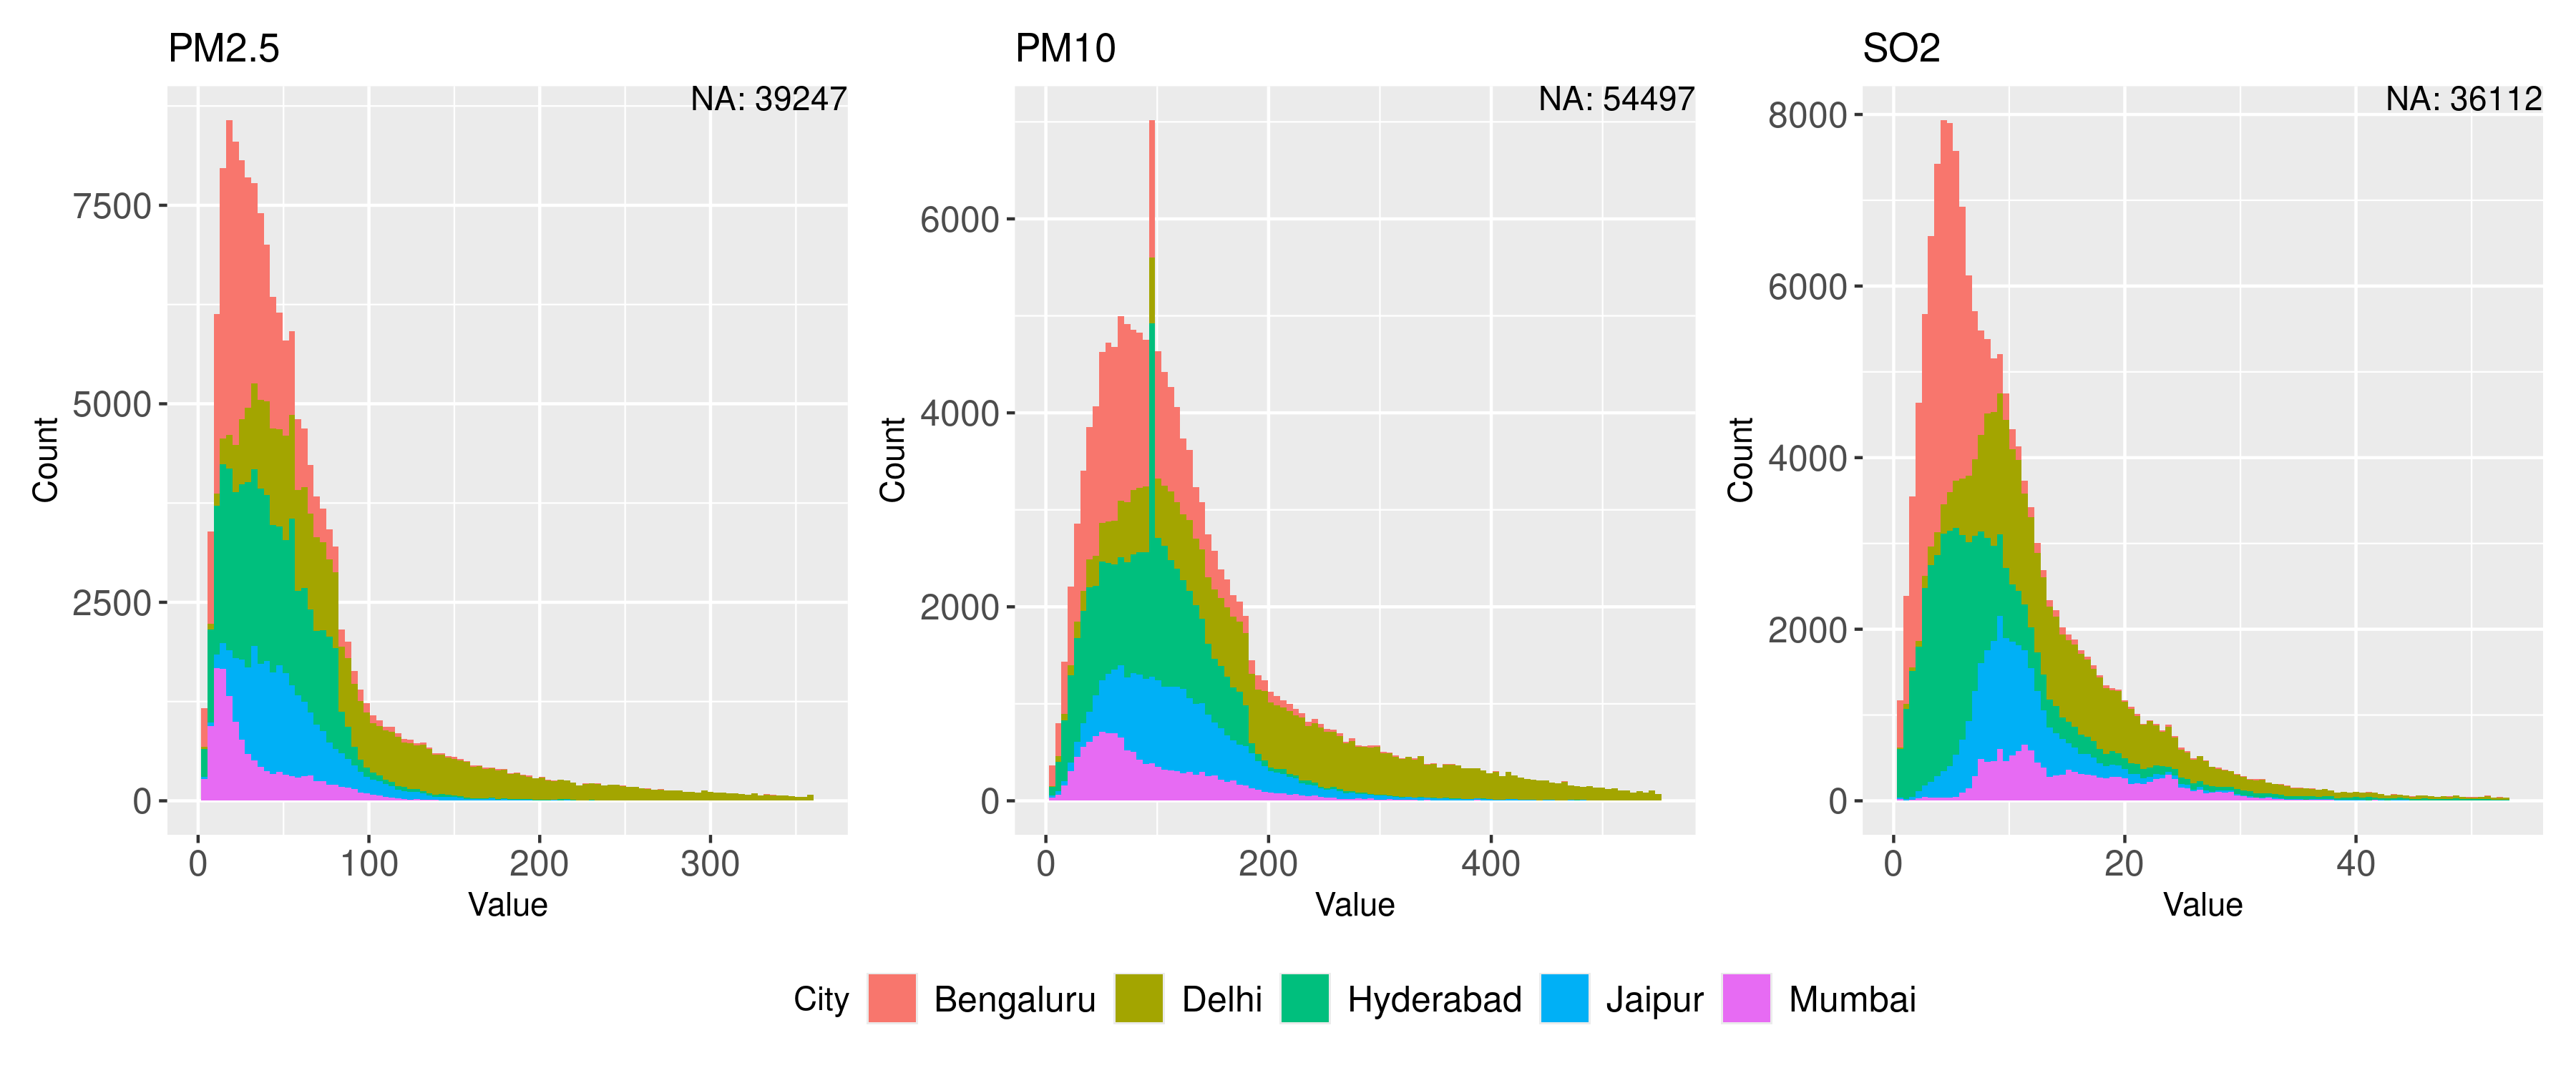
\includegraphics[width=\textwidth]{assets/skewness.png}
    \end{center}
    \vfill
\end{frame}

\begin{frame}{After Log Transformation}
    \begin{itemize}
        \item Applied $\log(1 + x)$ transformation to all outcome variables
            \begin{itemize}
                \item Resulted in more normal-like distributions
            \end{itemize}
    \end{itemize}
    \vspace{1em}
    \begin{center}
        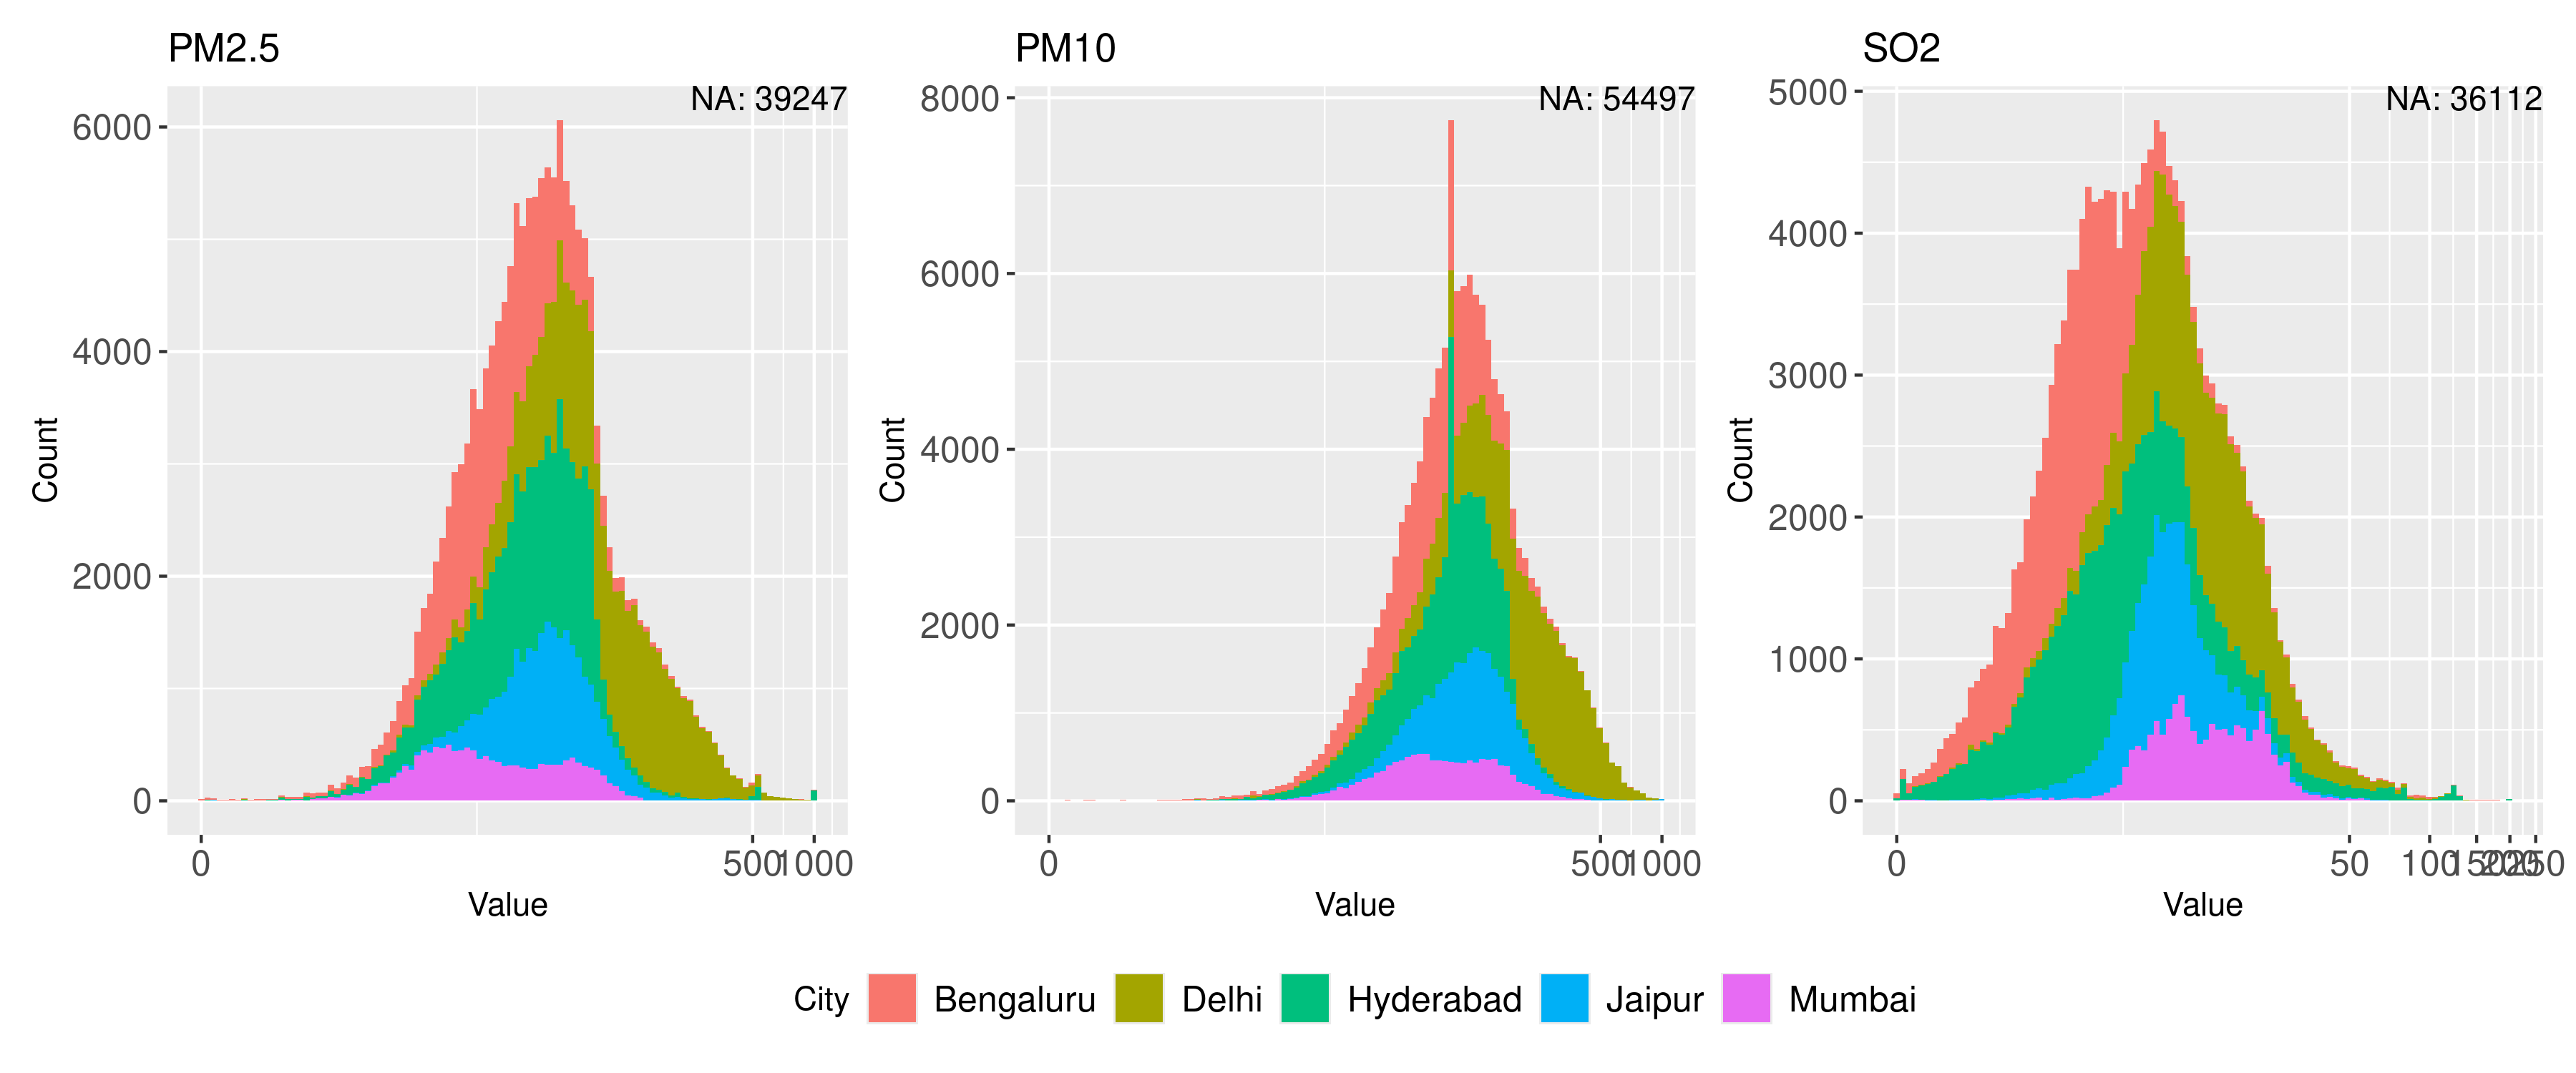
\includegraphics[width=\textwidth]{assets/log-scaled-pollutants.png}
    \end{center}
    \vfill
\end{frame}

\begin{frame}{Feature Engineering}
\begin{itemize}
    \item Temporal Features
        \begin{itemize}
            \item Hour of the day
                \begin{itemize}
                    \item Cosine/Sine features to capture cyclic (12 and 24-hour) patterns
                \end{itemize}
            \item Day of the week (categorical)
            \item Month of the year (categorical)
        \end{itemize}
    \item Weather-Related Features
        \begin{itemize}
            \item Wind components (X and Y axes)
            \item 24-hour cumulative precipitation and wind speed
        \end{itemize}
    \item All continuous features were scaled
\end{itemize}
\end{frame}

\begin{frame}{Preliminary Analysis}
    \vspace{0.5em}
    \begin{center}
        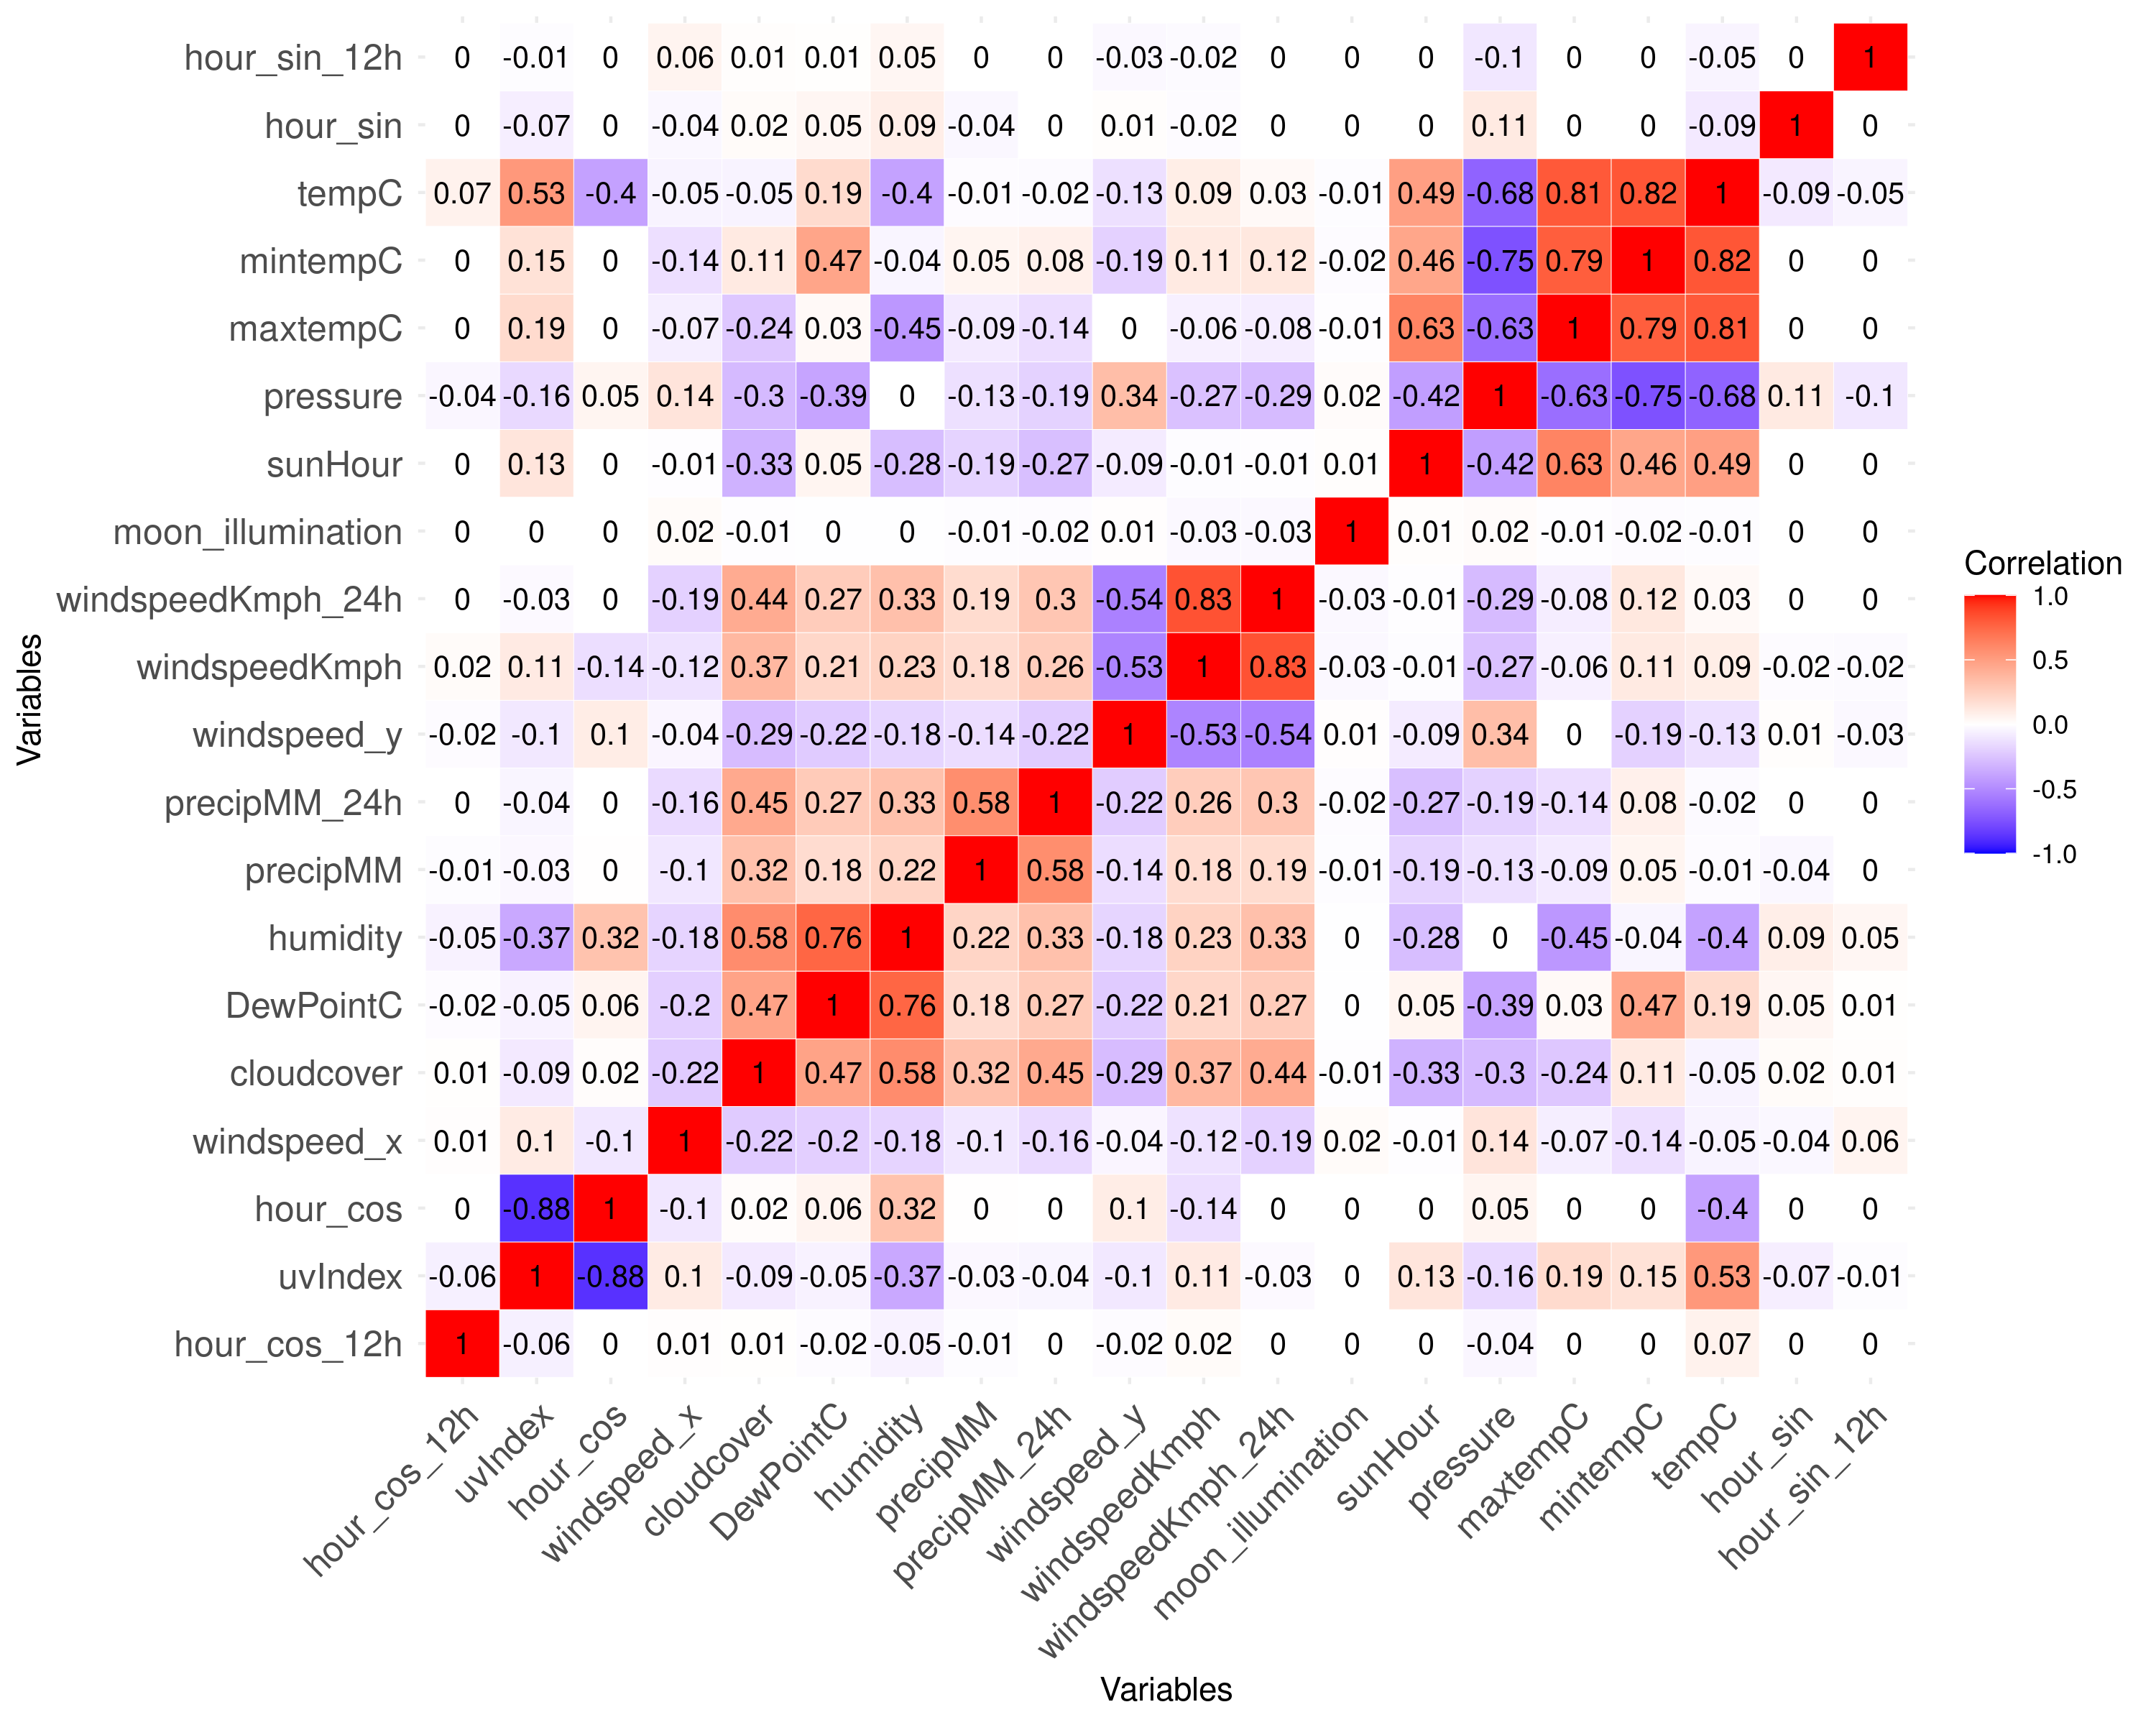
\includegraphics[width=0.84\textwidth]{assets/feature-correlation-matrix-final.png}
    \end{center}
    \vfill
\end{frame}

\begin{frame}{Preliminary Analysis}
    \begin{itemize}
       \item Weather correlations
           \begin{itemize}
               \item Humidity: negative with most pollutants
               \item Wind speed: negative with most pollutants, aids pollutant dispersion
               \item Temperature: positive with O\textsubscript{3}
               \item UV index: positive with O\textsubscript{3}
           \end{itemize}
       \item Significantly higher pollution in autumn and winter
       \item Pollution correlations
           \begin{itemize}
               \item Most pollutants positively correlated with each other
               \item O\textsubscript{3} shows distinct pattern from other pollutants
           \end{itemize}
    \end{itemize}
\end{frame}

\section{Methodology}

\begin{frame}{Model Development}
\begin{itemize}
    \item Independent linear regression models for each
        \begin{itemize}
            \item City
            \item Response variable
        \end{itemize}
    \item Data splitting
        \begin{itemize}
            \item Training: 2015-2018
            \item Testing: 2019
        \end{itemize}
    \item Removed features with VIF > 4
        \begin{itemize}
            \item minTempC
            \item maxTempC
            \item DewPointC
        \end{itemize}
\end{itemize}
\end{frame}

\begin{frame}{Model Performance (Mean per City/Pollutant)}
    \fontsize{11}{13}\selectfont
    \begin{table}
    \centering
    \begin{tabular}{lrrr}
    \hline
    Response & r & R\textsuperscript{2} & RMSE \\
    \hline
    PM2.5 & 0.728 & \textbf{0.538} & 0.437 \\
    PM10 & 0.694 & \textbf{0.492} & 0.435 \\
    O3 & 0.660 & \textbf{0.443} & 0.576 \\
    NOx & 0.430 & 0.214 & 0.604 \\
    NH3 & 0.338 & 0.161 & 0.420 \\
    CO & 0.311 & 0.132 & 0.307 \\
    SO2 & 0.273 & 0.102 & 0.388 \\
    \hline
    \end{tabular}
    \end{table}
    % \end{frame}
    
    % \begin{frame}{Model Performance by City}
    \begin{table}
    \centering
    \begin{tabular}{lrrr}
    \hline
    City & r & R\textsuperscript{2} & RMSE \\
    \hline
    Delhi & 0.615 & \textbf{0.403} & 0.412 \\
    Hyderabad & 0.598 & \textbf{0.390} & 0.390 \\
    Bengaluru & 0.427 & 0.246 & 0.481 \\
    Jaipur & 0.411 & 0.198 & 0.472 \\
    Mumbai* & 0.061 & 0.007 & 0.649 \\
    \hline
    \end{tabular}
    \end{table}
    \begin{center}
    \footnotesize{* Mumbai had substantial missing data, only 2/7 pollutants were modeled}
    \end{center}
\end{frame}

% \begin{frame}{Key Findings}
% \begin{itemize}
%     \item Best predictions for
%         \begin{itemize}
%             \item PM\textsubscript{2.5} (R\textsuperscript{2} = 0.538)
%             \item PM\textsubscript{10} (R\textsuperscript{2} = 0.492)
%             \item O\textsubscript{3} (R\textsuperscript{2} = 0.443)
%         \end{itemize}
%     \item Best performing cities
%         \begin{itemize}
%             \item Delhi (R\textsuperscript{2} = 0.403)
%             \item Hyderabad (R\textsuperscript{2} = 0.390)
%         \end{itemize}
% \end{itemize}
% \end{frame}

\section{Conclusion}

\begin{frame}{Conclusions}
\begin{itemize}
    \item Models show moderate predictive power
        \begin{itemize}
            \item R\textsuperscript{2} between 0.006 and 0.672, mean = 0.292
            \item Varies significantly across pollutants and cities
        \end{itemize}
    \item Key predictors
        \begin{itemize}
            \item Month of the year
            \item Humidity (negative link)
            \item Temperature (positive link)
            \item $\cos(hour\ of\ day)$
            \item Precipitation over 24 hours
        \end{itemize}
    \item Temporal patterns are strong predictors
    \item Meteorological variables show consistent influence
\end{itemize}
\end{frame}

\begin{frame}{Room for Improvement}
\begin{itemize}
    \item Explore more sophisticated approaches
        \begin{itemize}
            \item Non-linear models
            \item Time series models (e.g. LSTM)
        \end{itemize}
    \item Additional predictors
        \begin{itemize}
            \item Satellite data
            \item Traffic information
            \item Industrial activity metrics
            \item Special events data
        \end{itemize}
    \item Extend to more cities and longer time periods
\end{itemize}
\end{frame}


\begin{frame}
\begin{center}
\LARGE
\color{mifcolor} Thank you for your attention
\end{center}
\end{frame}

\end{document}